\documentclass[crop, tikz]{standalone}
\usepackage{tikz}

% Colour
\usepackage{xcolor}
\colorlet{LightCyan}{cyan!30}
\colorlet{LightLime}{lime!40}
\colorlet{LightGray}{lightgray!30}
\colorlet{FadedBlack}{black!40}
% Nodes
\tikzstyle{LSTMblock}=[draw,fill=LightCyan,minimum size=20pt,inner sep=1pt]
\tikzstyle{invisNode}=[circle, line width=0mm, inner sep=0pt]
\tikzstyle{stateTransition}=[-stealth, thick]
\tikzstyle{dotted}=[line width=1pt, dash pattern=on \pgflinewidth off 6pt]
\tikzstyle{sumNode}=[draw,circle,fill=LightLime,minimum size=20pt,inner sep=1pt]
\tikzstyle{ConcatBlock}=[draw,fill=LightGray,minimum size=20pt,inner sep=1pt]
% Reverse direction vector arrow
\usepackage{graphicx}
\newcommand{\cev}[1]{\reflectbox{\ensuremath{\vec{\reflectbox{\ensuremath{#1}}}}}}

\begin{document}
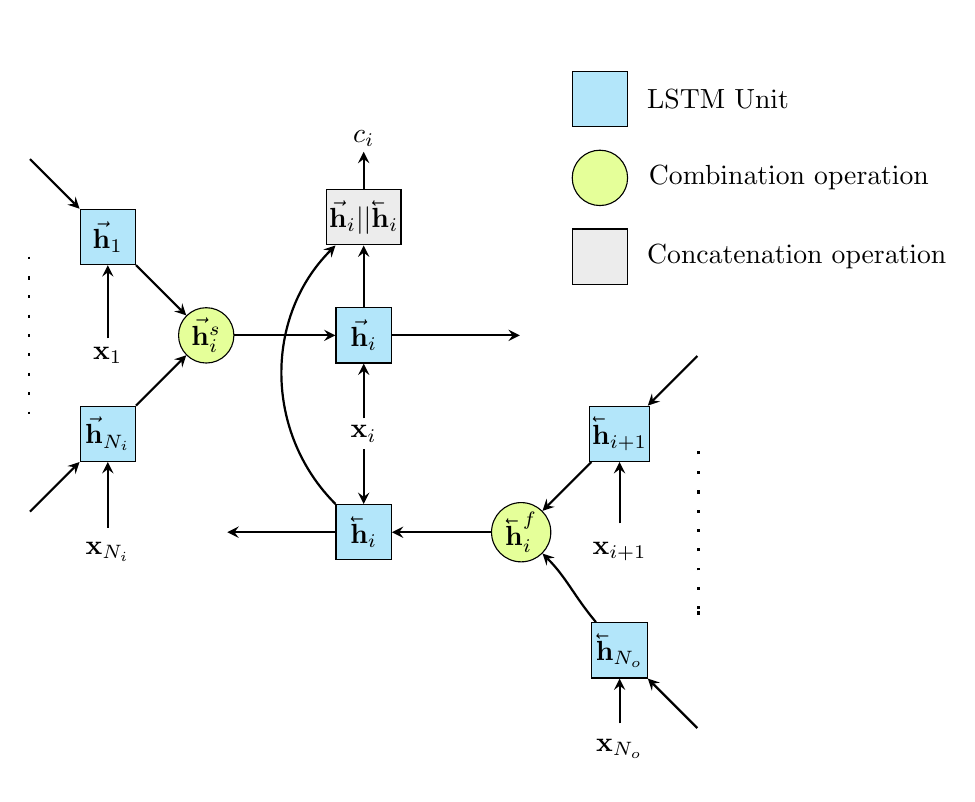
\begin{tikzpicture}
    % Incoming layer
    \node[invisNode] (invis1) at (-5.25,2.25) {};
	\node[LSTMblock] (h0) at (-4.25, 1.25) {$\vec{\mathbf{h}}_{1}$};
	\node[invisNode] (x0) at (-4.25, -0.25) {$\mathbf{x}_{1}$};
	\draw[stateTransition] (invis1) to[out=315,in=135] node [midway, sloped, above] {} (h0);
	\draw[stateTransition] (x0) to[out=90,in=270] node [midway, sloped, above] {} (h0);

    \node[invisNode] (invis2) at (-5.25,-2.25) {};
	\node[LSTMblock] (h1) at (-4.25, -1.25) {$\vec{\mathbf{h}}_{N_i}$};
	\node[invisNode] (x1) at (-4.25, -2.75) {$\mathbf{x}_{N_i}$};
	\draw[stateTransition] (invis2) to[out=45,in=225] node [midway, sloped, above] {} (h1);
	\draw[stateTransition] (x1) to[out=90,in=270] node [midway, sloped, above] {} (h1);

	\draw[dotted] (-5.25, 1.0) to[out=270,in=90] node [midway, sloped, above] {} (-5.25, -1.0);

	\node[sumNode] (h2) at (-3, 0) {$\vec{\mathbf{h}}_i^s$};
	\draw[stateTransition] (h1) to[out=45,in=225] node [midway, sloped, above] {} (h2);
	\draw[stateTransition] (h0) to[out=315,in=135] node [midway, sloped, above] {} (h2);
	
	\node[LSTMblock] (h3) at (-1, 0) {$\vec{\mathbf{h}}_{i}$};
	\node[invisNode] (h4) at (1, 0) {};
	\draw[stateTransition] (h2) to[out=0,in=180] node [midway, sloped, above] {} (h3);
	\draw[stateTransition] (h3) to[out=0,in=180] node [midway, sloped, above] {} (h4);
	\node[invisNode] (x2) at (-1, -1.25) {$\mathbf{x}_{i}$};
	\draw[stateTransition] (x2) to[out=90,in=270] node [midway, sloped, above] {} (h3);

	\node[LSTMblock] (h5) at (-1, -2.5) {$\cev{\mathbf{h}}_{i}$};
	\draw[stateTransition] (x2) to[out=270,in=90] node [midway, sloped, above] {} (h5);
	\node[ConcatBlock] (h6) at (-1, 1.5) {$\vec{\mathbf{h}}_{i}||\cev{\mathbf{h}}_{i}$};
	\draw[stateTransition] (h3) to[out=90,in=270] node [midway, sloped, above] {} (h6);
	\draw[stateTransition] (h5) to[out=135,in=225] node [midway, sloped, above] {} (h6);
    \node[invisNode] (invis5) at (-2.75, -2.5) {};
	\draw[stateTransition] (h5) to[out=180,in=0] node [midway, sloped, above] {} (invis5);


	\node[sumNode] (h9) at (1, -2.5) {$\cev{\mathbf{h}}_i^f$};
	\draw[stateTransition] (h9) to[out=180,in=0] node [midway, sloped, above] {} (h5);
	\node[LSTMblock] (h10) at (2.25, -4) {$\cev{\mathbf{h}}_{N_o}$};
	\node[LSTMblock] (h11) at (2.25, -1.25) {$\cev{\mathbf{h}}_{i+1}$};
	\draw[stateTransition] (h10) to[out=130,in=315] node [midway, sloped, above] {} (h9);
	\draw[stateTransition] (h11) to[out=225,in=45] node [midway, sloped, above] {} (h9);
	\node[invisNode] (x3) at (2.25, -5.25) {$\mathbf{x}_{N_o}$};
    \node[invisNode] (x4) at (2.25, -2.75) {$\mathbf{x}_{i+1}$};
	\draw[stateTransition] (x3) to[out=90,in=270] node [midway, sloped, above] {} (h10);
	\draw[stateTransition] (x4) to[out=90,in=270] node [midway, sloped, above] {} (h11);

	\node[invisNode] (h7) at (-1, 2.5) {$c_{i}$};
	\draw[stateTransition] (h6) to[out=90,in=270] node [midway, sloped, above] {} (h7);

    \node[invisNode] (invis3) at (3.25,-0.25) {};
	\draw[stateTransition] (invis3) to[out=225,in=45] node [midway, sloped, above] {} (h11);
    \node[invisNode] (invis4) at (3.25,-5.0) {};
	\draw[stateTransition] (invis4) to[out=135,in=315] node [midway, sloped, above] {} (h10);
	\draw[dotted] (3.25, -3.5) to[out=270,in=90] node [midway, sloped, above] {} (3.25, -1.5);

% Legend
\node[LSTMblock] (LSTMLegend) at (2, 3) {};
\node[invisNode] (LSTMtext) at (3.5,3) {LSTM Unit};
\node[sumNode] (sumLegend) at (2, 2) {};
\node[invisNode] (LSTMtext) at (4.4,2) {Combination operation};
\node[ConcatBlock] (concatLegend) at (2, 1) {};
\node[invisNode] (LSTMtext) at (4.5,1) {Concatenation operation};

\end{tikzpicture}

\end{document}